\documentclass{report}

\usepackage[ngerman]{babel}
\usepackage[utf8]{inputenc}
\usepackage[T1]{fontenc}
\usepackage{hyperref}
\usepackage{csquotes}
\usepackage[a4paper]{geometry}
\usepackage{graphicx} %Um externe Bilddateien einfügen zu können.
\usepackage{float}
\usepackage{caption}

\usepackage[
    backend=biber,
    style=apa,
    sortlocale=de_DE,
    natbib=true,
    url=false,
    doi=false,
    sortcites=true,
    sorting=nyt,
    isbn=false,
    hyperref=true,
    backref=false,
    giveninits=false,
    eprint=false]{biblatex}
\addbibresource{../references/bibliography.bib}


\title{Ethik im Umgang mit Daten}
\author{Latisha Soares de Carvalho}
\date{30.05.2024}


\begin{document}

% Hier wird die Titelseite gestaltet.
\begin{titlepage}
    \makeatletter % Das hier brauchen wir damit wir spezielle Befehle wie \@author verwenden können.
	\begin{center}
		{\scshape Gymnasium Muttenz} \vspace{0.5cm}

		 Informatik 2023/2024\vspace{5.5cm}

		{\huge\bfseries \@title}

        \vspace{1cm}

        \begin{figure}[h]
            \centering 
            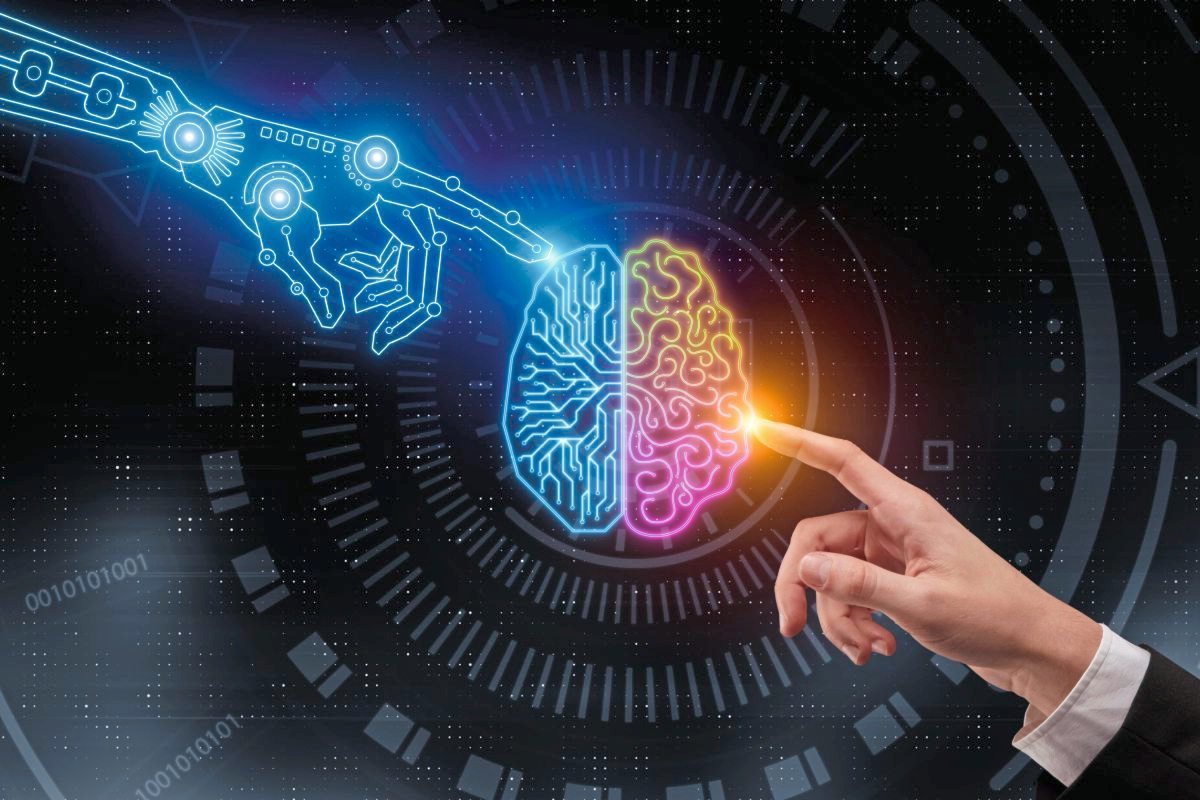
\includegraphics[width=0.5\textwidth]{KI.jpg} 
            %\caption{Ein erstes Bild}
            %\label{fig:meme}
            \end{figure}

		\vspace{2cm}

		{\Large\itshape \@author}

        \vspace{2cm}

        Version vom: \@date
	\end{center}
    
    \makeatother % Wir müssen das @ wieder schliessen, damit der Rest ganz normal funktioniert.
\end{titlepage}

\abstract{
    In diesem Projekt verstehe ich die Ethik im Umgang mit Daten.
    Daher versuche ich es durch eine eigene Fragestellung Ihnen, den Lesern, zu übermittteln. Und Ihnen,
    somit einer der Fragen, die Sie selbst sich möglicherweise gestellt haben, auf zu klären.
}

\tableofcontents

\chapter{Einleitung}
Die Einführung in das KI-Training beginnt mit dem Sammeln der Daten in einem Computersystem, dass Daten Vorhersagen trifft und deren Genauigkeit bewertet.
 Techniken des maschinellen Lernens, einschließlich Deep Learning, können verwendet werden, um Daten zu analysieren und zu verbessern. 
    Dieser Trainingsprozess ermöglicht es der Software, Merkmale in Daten zu erkennen und sich ständig zu verbessern.
    
    Es gibt zwei Hauptmethoden zum Trainieren von KI: überwachtes und unüberwachtes Lernen.
    Beim überwachten Lernen werden gekennzeichnete Daten für das Training verwendet, während beim unüberwachten Lernen das Modell von Mustern in unbeschrifteten Daten verwendet wird.
    
    Der nächste Schritt des Trainingsprozesses ist die Validierung. Dabei wird die Leistung des Modells anhand unabhängiger Modelle bewertet, um festzustellen, ob das Training angepasst werden muss.
    Dazu gehört die Bewertung der Leistung des Modells im Vergleich zu unabhängigen Modellen, um festzustellen, ob das Training angepasst werden muss. 

    Nach der Validierung folgt die Prüfung, bei dem das Modell auf unstrukturierte Daten verwendet wird, um seine Echtheit in der realen Welt nachzuprüfen.
    Mögliche Probleme wie Überanpassung oder Unteranpassung müssen berücksichtigt werden und das Modell sollte falls nötig angepasst werden.

    Das KI-Training erfordert mehrere Faktoren, darunter die Datenqualität, die Software und Verfügbarkeit.
    Eine sorgfältige Planung und Durchführung des Prozesses ist für die Entwicklung einer erfolgreichen und geeigneten KI-Modells notwendig.

    \section {Was ist KI?}
    Die Künstliche Intelligenz, auch abgekürzt KI genannt, ist die Begabung einer Maschine, menschliches Verhalten wie sinnvolles Denken, Lernen, Organisieren und Kreativität, per Software auf einen Computer zu übertragen. Der Computer lernt anhand der KI selbständig Entscheidungen zu treffen, Antworten zu finden und Probleme zu lösen.

\chapter{Beantwortung der Frage}

\section {Fragestellung}
Wer trägt die Verantwortung, wenn ein KI-System fehlerhafte oder unethische Entscheidungen trifft?

\section {Einführung zu meinem Thema}
In einer Welt voller KI stellt sich eine wichtige Frage: Wer ist verantwortlich, 
wenn ein KI-System falsche oder unethische Entscheidungen trifft? 
Stellen Sie sich vor, Sie gehen zum Arzt und werden dort falsch diagnostiziert, da der Doktor ein KI-System verwendet hat. Wer trägt nun die Verantwortung? Ist es der Arzt, der die künstliche Intelligenz benutzt hat, Ist es der Hersteller des KI-Systems oder das Krankenhaus, welches erlaubt hat, die neue Technologie einzuführen?
Oder denken Sie an selbstfahrende Autos, die vor schwierigen Entscheidungen stehen. Wer ist verantwortlich, wenn das Auto eine unerwartete Entscheidung trifft? Diese Beispiele zeigen, dass wir klare Regeln brauchen, um festzulegen, wer verantwortlich ist, wenn KI-Systeme Probleme haben. 

\section{Haftungsverpflichtung}
Die Haftung für Schäden, die durch KI-Entscheidungen verursacht werden, ist unklar und hängt von vielen Faktoren ab, wie z.B. die beteiligten Parteien, bestehenden Verträgen, nationaler und internationaler Gesetzgebung, zu dem noch die technischen Eigenschaften der KI-Systeme. In der Technik wird es häufig eine Kombination von Verantwortlichkeiten des Entwicklers, des Betreibers und vielleicht des Benutzers geben, abhängig von den konkreten Umständen des Falls und den geltenden rechtlichen Rahmenbedingungen.

\subsection{Verantwortlichkeit der Entwickler und Hersteller}

\begin{itemize}
    \item Produkthaftung: Entwickler und Hersteller von KI könnten haftbar gemacht werden, wenn ein Defekt in der Software oder Hardware bezeugt wird. Dies könnte unter die Produkthaftungsgesetze fallen, die für inkorrekte Produkte gelten.
    \item Sorgfaltspflicht: Wenn nachgeprüft werden kann, dass die Entwickler oder Hersteller ihrer Pflicht nicht berücksichtigt haben, z.B. aufgrund mangelhafter Tests oder unzureichende Schutzmassnahmen, könnten sie haftbar gemacht werden.
\end{itemize}
		
\subsection{Verantwortlichkeit der Betreiber und Nutzer}

\begin{itemize}
\item Haftung der Nutzer: Unternehmen oder Einzelpersonen, die KI-Systeme betreiben, könnten haftbar sein, wenn sie diese Systeme unprofessionell nutzen oder wenn sie keine Schutzmechanismen, angemessene Überwachung und Kontrolle einsetzen. 
\item Vertragliche Haftung: Wenn zwischen dem Nutzer und dem Entwickler ein Vertrag besteht, können die Fragen der Verantwortlichkeit auch durch die bestimmten Bestimmungen des Vertrags geregelt werden.
\end{itemize}

\subsection{Gemeinsame Verantwortung}
\begin {itemize}
\item Haftungsteilung: In einigen Fällen könnte es zu einer gemeinsamen Verantwortung führen, bei der sowohl Entwickler als auch Inhaber zu unterschiedlichen Verhältnissen haftbar gemacht werden. Dies kann besonders bei komplizierten Systemen so sein, bei denen verschiedene Parteien an der Entstehung und dem Betrieb beteiligt sind.
\end{itemize}

\subsection{Künstliche Intelligenz und autonome Systeme} 
\begin{itemize}
    \item Haftung für autonome Entschlüsse: Bei autonomen Systemen, die Entscheidungen ohne menschliches Eingreifen treffen, ist die Frage, wer dafür verantwortlich ist, besonders schwierig. Hier diskutieren die Juristen und Gesetzgeber, eine einfache Lösung, um diese Herausforderung zu umgehen. Die folgenden Ideen, die sie bereits haben lauten z.B. die Einführung eines neuen rechtlichen Status für autonome Systeme oder spezielle Versicherungslösungen.
\end{itemize}


\chapter{Fazit}

Die Durchführung von KI bringt auf der einen Seite wichtige Vorteile mit sich, stellt jedoch auf der anderen Seite vielfältige Haftungsfragen dar. Oft gibt es keine deutlichen Verantwortlichkeiten, die sich auf Entwickler, Hersteller, Betreiber und Nutzer beziehen. Es besteht die Option, dass Entwickler aufgrund von Produkthaftung und Sorgfaltspflicht haftbar sind, während Betreiber und Nutzer bei amateurhafter Nutzung zur Rechenschaft gezogen werden können. Die Haftung autonomer Systeme, die ohne menschliche Einmischung handeln, ist besonders anspruchsvoll. Um die Entscheidungsbefugnis festzulegen und die sichere Anwendung von KI zu erfüllen, sind spezifische gesetzliche Rahmenbedingungen und eventuelle Lösungen wie neue rechtliche Entwicklungsstände oder spezielle Versicherungen nötig.


\nocite{*}
\printbibliography
\end{document}

\input{chap_methode.tex} 






